\documentclass[8pt]{beamer}
\mode<presentation>
\ProcessOptionsBeamer
\useoutertheme[footline=authorinstitutetitle,subsection=false]{smoothbars}
\makeatletter 
\newcommand{\frameofframes}{/}
\newcommand{\setframeofframes}[1]{\renewcommand{\frameofframes}{#1}}
\setbeamertemplate{footline} 
  {%
    \begin{beamercolorbox}[colsep=1.5pt]{upper separation line foot}
    \end{beamercolorbox}
    \begin{beamercolorbox}[ht=2.5ex,dp=1.125ex,%
      leftskip=.3cm,rightskip=.3cm plus1fil]{author in head/foot}%
      \leavevmode{\usebeamerfont{author in head/foot}\insertshortauthor}%
      \hfill%
      {\usebeamerfont{institute in head/foot}\usebeamercolor[fg]{institute in head/foot}\insertshortinstitute}%
    \end{beamercolorbox}%
    \begin{beamercolorbox}[ht=2.5ex,dp=1.125ex,%
      leftskip=.3cm,rightskip=.3cm plus1fil]{title in head/foot}%
      {\usebeamerfont{title in head/foot}\insertshorttitle}%
      \hfill%
      {\usebeamerfont{frame number}\usebeamercolor[fg]{frame number}\insertframenumber~\frameofframes~\inserttotalframenumber}
    \end{beamercolorbox}%
    \begin{beamercolorbox}[colsep=1.5pt]{lower separation line foot}
    \end{beamercolorbox}
  }
\makeatother
\hypersetup{
    urlcolor=blue 
}
\useinnertheme{circles}
\usepackage{multirow}
\usepackage{graphicx}
\usepackage{algorithm}
\usepackage{algpseudocode}
\setlength{\columnseprule}{0.3pt}
\xdefinecolor{cuhksz1}{rgb}{0.457,0.0585,0.42578}      %RGB(117,15,109)
\xdefinecolor{cuhksz2}{rgb}{0.86328,0.63671875,0}      %RGB(221,163,0)
\xdefinecolor{cuhksz3}{rgb}{0.953125,0.87109,0.6875}   %RGB(244,223,176)
\setbeamercolor{footline}{bg=cuhksz1}
\setbeamercolor{frametitle}{bg=cuhksz1,fg=cuhksz3}
\setbeamercolor{title}{bg=cuhksz1}
\setbeamerfont{frametitle}{size=\large}
\setbeamertemplate{bibliography item}[text]
\setbeamertemplate{caption}[numbered]
\setbeamercolor{palette primary}{use=structure,fg=cuhksz2,bg=structure.fg}
\setbeamercolor{palette secondary}{use=structure,fg=cuhksz2,bg=structure.fg!75!black}
\setbeamercolor{palette tertiary}{use=structure,fg=cuhksz2,bg=structure.fg!50!black}
\setbeamercolor{palette quaternary}{fg=cuhksz2,bg=structure.fg!50!black}
\setbeamercolor{titlelike}{parent=palette primary}
\setbeamercolor{block title}{bg=cuhksz1,fg=cuhksz3}
\setbeamercolor*{block title example}{use={normal text,example text},bg=cuhksz3,fg=cuhksz1}
\setbeamercolor{fine separation line}{}
\setbeamercolor{item projected}{fg=cuhksz3}
\setbeamercolor{palette sidebar primary}{use=normal text,fg=normal text.fg}
\setbeamercolor{palette sidebar quaternary}{use=structure,fg=structure.fg}
\setbeamercolor{palette sidebar secondary}{use=structure,fg=structure.fg}
\setbeamercolor{palette sidebar tertiary}{use=normal text,fg=normal text.fg}
\setbeamercolor{section in sidebar}{fg=cuhksz2}
\setbeamercolor{section in sidebar shaded}{fg=cuhksz3}
\setbeamercolor{separation line}{}
\setbeamercolor{sidebar}{bg=cuhksz1}
\setbeamercolor{sidebar}{parent=palette primary}
\setbeamercolor{structure}{fg=cuhksz1}
\setbeamercolor{subsection in sidebar}{fg=cuhksz2}
\setbeamercolor{subsection in sidebar shaded}{fg=cuhksz3}
\AtBeginSection[]{
	\begin{frame}
		\tableofcontents[sectionstyle=show/shaded,subsectionstyle=show/shaded/hide,subsubsectionstyle=show/shaded/hide]
	\end{frame}
}
\AtBeginSubsection[]{
	\begin{frame}
		\tableofcontents[sectionstyle=show/shaded,subsectionstyle=show/shaded/hide,subsubsectionstyle=show/shaded/hide]
	\end{frame}
}
\mode
<all>

\usepackage{graphicx}

\title{Algorithmic Collusion of Competitive Dynamic Pricing: Past, Present and Future}
\author{Chen Tang \inst{1}}
\institute{\inst{1}  School of Data Science, Chinese University of Hong Kong, Shenzhen}
\date{July 2024}
\begin{document}

\begin{frame}
    \titlepage
    \begin{figure}[htpb]
        \begin{center}
            
\includegraphics[width=0.3\linewidth]{pic/CUHKSZ-Logo.png}
        \end{center}
    \end{figure}
    \begin{center}
        \tiny {The paper for this presentation is available \href{https://papers.ssrn.com/sol3/papers.cfm?abstract_id=4891632}{\textcolor{red}{HERE}}.\\
        More information about the author can be found \href{https://chentang01.github.io/}{\textcolor{red}{HERE}}.}
    \end{center}
    
\end{frame}

\section{Introduction}

\begin{frame}{Introduction to Dynamic Pricing}
    Dynamic pricing studies how to adapt prices in response to demand fluctuations.
    \begin{columns}
        \begin{column}{0.48\textwidth}
            It's widely been used in industries:
            \begin{itemize}
                \item Electricity Market;
                \item Online Retailing;
                \item Airline Companies.
            \end{itemize}
            I recommend \cite{den2015dynamic} as a general review for dynamic pricing.
        \end{column}
        \begin{column}{0.48\textwidth}
            \begin{figure}
                \centering
                
\includegraphics[width=0.2\linewidth]{pic/mckinsey.png}
            \end{figure}
            \begin{enumerate}
                \item \large{2} to \large{5} percent growth in sales;
                \item \large{5} to \large{10} percent growth in profit margins.
            \end{enumerate}
            \begin{figure}
                \centering
                
\includegraphics[width=0.2\linewidth]{pic/BCG.png}
            \end{figure}
            \begin{itemize}
                \item It can lift consumer satisfaction during the purchasing.
            \end{itemize}
        \end{column}
    \end{columns}
\end{frame}

\begin{frame}{Dynamic Pricing under Competition}
    Most previous research has focused on three primary aspects:
    \vspace{1cm}
    \begin{enumerate}
        \item Given a competitive pricing environment, what is the theoretical equilibrium of the game? Is it unique or not?
        \begin{itemize}
            \item One-period / Multi-stage;
            \item Capacity / Inventory Constraint;
            \item Homogeneous / Heterogeneous Prodducts.
        \end{itemize}
        \item The validity of the \textit{market response hypothesis}:
        \begin{itemize}
            \item If both firms use a monopoly model to learn the environment, can the game converge to the equilibrium?
        \end{itemize}
        \item Strategy of dynamic pricing in a competitive environment.
    \end{enumerate}
    \vspace{1cm}
    The study of algorithmic collusion is a new subfield \textbf{\textcolor{cuhksz2}{only after 2020}}. 
\end{frame}

\begin{frame}{A taste on algorithmic collusion}
    \begin{columns}
        \begin{column}{0.48\textwidth}
            Using the prisoners dilemma as the toy model:
            \begin{table}[htbp]
                \centering
                \caption{The payoff matrix of the toy model}
                \label{tab:toy_payoff_matrix}
                \begin{tabular}{cc|c|c}
                    & & \multicolumn{2}{c}{Firm 2} \\
                    & & $H$ & $L$ \\
                    \hline
                    \multirow{2}{*}{Firm 1} & $H$ & $(2,2)$ & $(0.5,3)$ \\
                    \cline{2-4}
                    & $L$ & $(3,0.5)$ & $(1,1)$ \\
                \end{tabular}
            \end{table}
            \vspace{0.5cm}
            In the static game (one-period), the unique Nash equilibrium is both setting low prices.
            \vspace{0.5cm}
            \begin{center}
                The greatness of the competition.
            \end{center}
        \end{column}
        \begin{column}{0.48\textwidth}
            What if both firms use the RL algorithm (such as Q-learning) to determine their prices, and both firms set high prices? 
            \vspace{1cm}
            
            \cite{calvano2019algorithmic} first observed this phenomenon in 2019 and called this as \textbf{algorithmic collusion} (unrigorous definition).
        \end{column}
    \end{columns}
\end{frame}

\begin{frame}{One-shot Deviation Principle}
    \begin{columns}
        \begin{column}{0.48\textwidth}
            The same payoff matrix, but multi-stage:
            \begin{table}[htbp]
                \centering
                \caption{The payoff matrix of the toy model}
                \begin{tabular}{cc|c|c}
                    & & \multicolumn{2}{c}{Firm 2} \\
                    & & $H$ & $L$ \\
                    \hline
                    \multirow{2}{*}{Firm 1} & $H$ & $(2,2)$ & $(0.5,3)$ \\
                    \cline{2-4}
                    & $L$ & $(3,0.5)$ & $(1,1)$ \\
                \end{tabular}
            \end{table}
            \vspace{0.5cm}
            In the dynamic game, the SPNE is not unique.
            \vspace{0.5cm}
            
            Collusion can be sustained if both firms use the one-shot deviation principle.
        \end{column}
        \begin{column}{0.48\textwidth}
            Assume the discount rates are $\delta_1$ and $\delta_2$ respectively, a reliable threat can exist if:
            \vspace{0.2cm}
            \[
        	\begin{aligned}
        		2\cdot \sum_{t=0}^\infty\delta_1^t &\ge 3 + 1 \cdot \sum_{t=1}^\infty \delta_1^t \\
        		2\cdot \sum_{t=0}^\infty\delta_2^t &\ge 3 + 1 \cdot \sum_{t=1}^\infty \delta_2^t \\
        		\delta_1 \ge \frac{2}{3} &, \delta_2 \ge \frac{2}{3}
        	\end{aligned}
            \] 
            \vspace{0.2cm}
            \textit{Folk Theorem}: collusion can occur as long as players are patient enough.
        \end{column}
    \end{columns}
\end{frame}

\begin{frame}{Spurious Collusion \& Genuine Collusion}
    A reliable collusion should exhibit a reward-punishment mechanism for the opponent's deviations.
    \vspace{0.5cm}
    
    \cite{calvano2023algorithmic} categorizes algorithmic collusion into two types:
    \begin{itemize}
    	\item \textit{Genuine Collusion}: High prices are the result of firms not recognizing the potential for greater short-term profits through deviation, rather than due to an explicit reward-punishment scheme.
    	\item \textit{Spurious Collusion}: High prices are maintained through a reward-punishment mechanism where the AI algorithm exhibits behavior akin to the one-shot deviation principle.
    \end{itemize}
    \begin{figure}
        \centering
        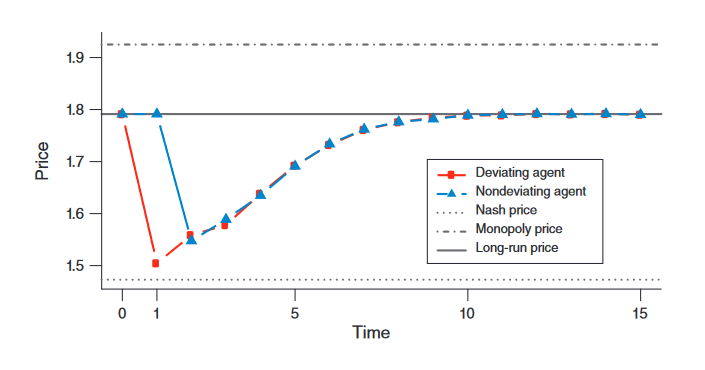
\includegraphics[width=0.5\linewidth]{pic/calvano_pic4.png}
        \caption{\\ \tiny This figure is from figure 4 in \cite{calvano2020artificial}.}
    \end{figure}
\end{frame}

\begin{frame}{Authentic Collusion}
    There are many critics on these findings, the most representative voice is:
    \vspace{0.2cm}

    \begin{itemize}
        \item Even though genuine collusion demonstrates a reward-punishment scheme to deviations, it can be outperformed (hacked) by other algorithms. Thus, this is not really `spurious'.
    \end{itemize}
    
    \vspace{0.2cm}
    Arnoud V. den Boer gives a rigorous definition of collusion, and I summarize it as the authentic collusion:
    \begin{itemize}
	\item \textit{Authentic Collusion}: collusion sustained by a theoretically reliable threat, and the collusive algorithm performs well enough against the opponent's alternative algorithms.
    \end{itemize}

    \begin{center}
        \textcolor{red}{These definitions are not just tautology!}
    \end{center}
\end{frame}

\begin{frame}{The directions of research on algorithmic collusion}
    The research on algorithmic collusion can be broadly categorized into two streams based on different directions:
    \vspace{0.3cm}
    \begin{enumerate}
    	\item This stream of research focuses on \textbf{convergence}, investigating whether specific AI algorithms could converge to spurious collusion, genuine collusion, or merely competitive outcomes.
    	\item This stream of research focuses on \textbf{equilibrium}, studying whether a specific algorithmic environment could formulate a collusive equilibrium. 
    \end{enumerate}
    \vspace{0.3cm}
    The \textit{convergence} and \textit{equilibrium} are not the same concepts. In many numerical experiments, the game can converge to a scenario that is not any equilibrium.
\end{frame}

\begin{frame}{Why Does Algorithmic Collusion Matter?}
    It's about the fairness of competition, a fair market can bring better welfare for the society.

    \vspace{1.5cm}

    Collusion is usually illegal (anti-monopoly law) in most regions, but using reinforcement learning may collude in a legal way.

    \vspace{1.5cm}
    Another realistic concern is that more and more companies are trying to use AI to price their products (\cite{spann2024algorithmic}).
\end{frame}

\section{Algorithmic Collusion under RL}

\begin{frame}{Introdution on Reinforcement Learning: Q-learning 1}
    Five key elements of reinforcement learning (in the context of dynamic pricing):
    \begin{enumerate}
	\item States ($\mathcal{S}$): a finite set representing all possible states of the environment (the firms' historical prices);
	\item Actions ($\mathcal{A}(\mathcal{S})$): a finite set of actions available to the decision-maker, which may depend on the current state (prices to be determined);
	\item Transition Probabilities ($\mathcal{T}:\mathcal{S}\times\mathcal{A}\to \mathcal{S}$): The probability of transitioning to a new state given the current state and the action taken (updated historical prices);
	\item Rewards Function ($\mathcal{R}:\mathcal{S}\times\mathcal{A}\to \mathbb{R}$): A function that assigns a reward for each state-action pair (revenue);
	\item Discount Factor ($\delta\in[0,1]$):  A factor that discounts future rewards based on their distance from the present.
    \end{enumerate}
    \vspace{0.2cm}
    A very famous algorithm is called \textbf{Q-learning}, which maintains a Q-function $Q(s,a)$ for every state-action pair:
    \begin{itemize}
        \item At each time $t$ given the current state $s_t$, the algorithm has two options:
        \begin{enumerate}
            \item With prob $\epsilon$: randomly pick an action from $\mathcal{A}$;
            \item With prob $1-\epsilon$: select $\arg\max_a Q(s_t,a)$;
        \end{enumerate}
        \item Note that $\epsilon$ is usually a decreasing function on $t$;
        \item Then the agent receives reward $r_{it}$ from the environment.
    \end{itemize}
\end{frame}

\begin{frame}{Introdution on Reinforcement Learning: Q-learning 2}
    \begin{figure}
        \centering
        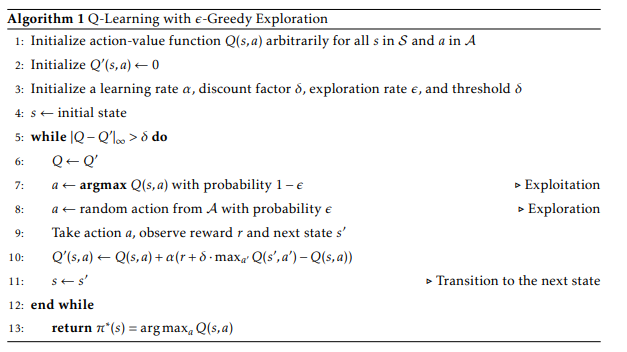
\includegraphics[width=0.7\linewidth]{pic/Q-learning.png}
    \end{figure}
    Most of the RL algorithms use a value function approximation scheme:
    \vspace{0.5cm}
    \begin{itemize}
        \item They maintain the Q-matrix for all state-action pairs;
        \item Use different approaches to estimate the Q-matrix (deep learning, sampling, etc)
    \end{itemize}
\end{frame}

\begin{frame}{Introdution on Reinforcement Learning: Bandit Learning}
    There is a type of \textit{state-free} algorithm called the bandit algorithm.
    \vspace{1cm}

    \begin{columns}
        \begin{column}{0.48\textwidth}
            \begin{itemize}
                \item Only maintaining the value function for the action space $Q(a)$ rather than $Q(s,a)$.
            \end{itemize}
        \end{column}
        \begin{column}{0.48\textwidth}
            UCB(upper confidence bound) algorithm:
            \[\begin{aligned}
                v_{a,t}&=\frac{1}{N_{a,t-1}}\sum_{t^{\prime}\leq t-1}r_{t^{\prime}}1\left\{a_{t^{\prime}}=a\right\}\\ &+\sqrt{\frac{2\log(1/\delta)}{N_{a,t-1}}}
            \end{aligned}\]
        \end{column}
    \end{columns}

    \vspace{0.5cm}
    Besides the value-based algorithms, policy gradient algorithms are proposed without relying on the estimation of the value function.
\end{frame}

\begin{frame}{Algorithmic Collusion: The initial paper 1}
    The first paper on algorithmic collusion is \cite{calvano2020artificial}. Assume there are $n$ different agents, the demand for firm $i$ at time $t$ is:
    \begin{equation}
        d_{i,t}=\frac{e^{\frac{a_i-p_{i,t}}\mu}}{\sum_{j=1}^ne^{\frac{a_j-p_{j,\iota}}\mu}+e^{\frac{a_0}\mu}}，
    \end{equation}
    They discretize the firms' action spaces: for each firm, we can compute its one-shot Bertrand-Nash equilibrium (\textbf{com}petitive price) $p^{com}$ and the monopoly (\textbf{col}lusive) price $p^{col}$. Then, taking the interval $[p^{com}-\xi(p^{col}-p^{com}), p^{col}+\xi(p^{col}-p^{com})], \xi>0$, and splitting the interval into $m$ discrete prices, we can get the action space for each agent. The state space is defined as the prices in the last $k$ epochs. Each agent utilizes the Q-learning algorithm to make decisions.
    \vspace{0.5cm}
    
    In the baseline experiment, $k=1, m=3$, and only two firms are competing.
\end{frame}

\begin{frame}{Algorithmic Collusion: The initial paper 2}
    The authors define the \textbf{average profit gain} $\Delta$:
    \[\Delta\equiv\frac{\bar{\pi}-\pi^{com}}{\pi^{col}-\pi^{com}}\]
    \begin{itemize}
        \item When $\Delta$ nears $1$, the game is in collusive scenario; when it nears $0$, the game is in competitive scenario;
        \item The left figure shows the Q-learning would converge to the collusive scenario, and the middle figure is my replication;
        \item The right figure shows that the agent can respond strategically to the opponent's deviation, meaning it's a genuine collusion.
    \end{itemize}
    \begin{columns}
        \begin{column}{0.33\textwidth}
            \begin{figure}
                \centering
                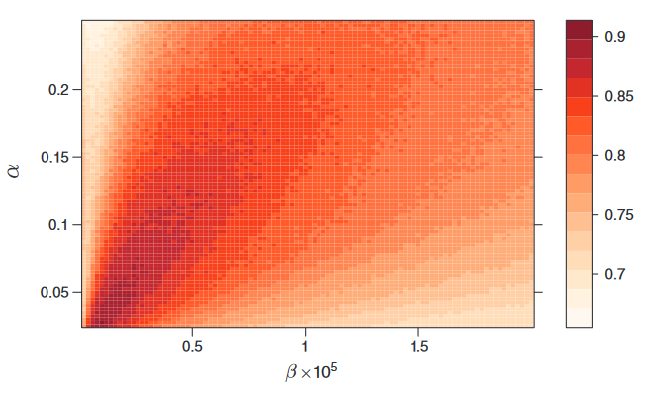
\includegraphics[width=0.99\linewidth]{pic/calvano_pic1.png}
            \end{figure}
        \end{column}
         \begin{column}{0.33\textwidth}
            \begin{figure}
                \centering
                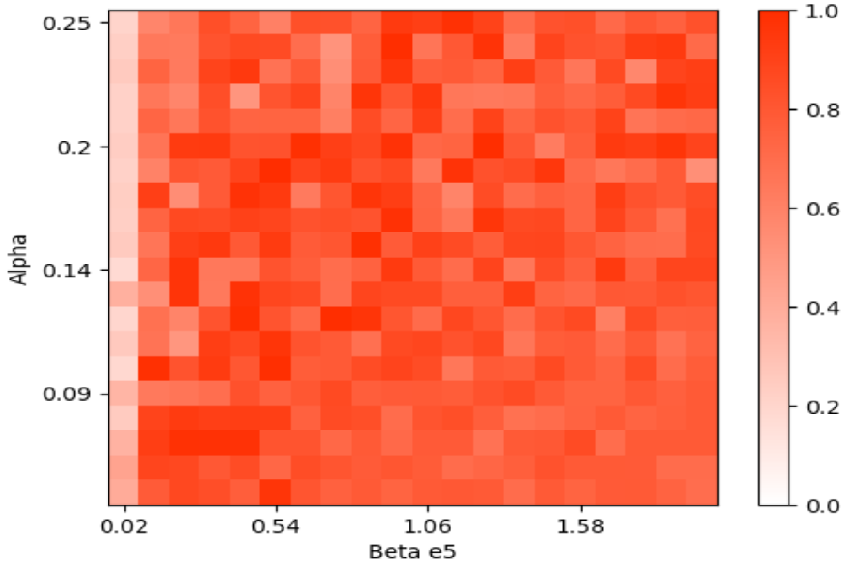
\includegraphics[width=0.9\linewidth]{pic/calvano_pic1_rep.png}
            \end{figure}
        \end{column}
        \begin{column}{0.34\textwidth}
            \begin{figure}
                \centering
                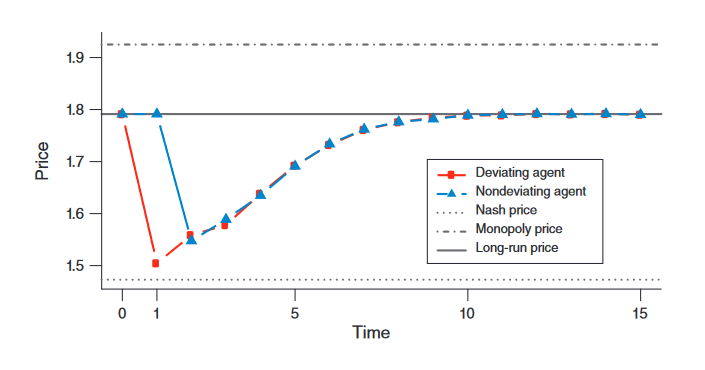
\includegraphics[width=0.99\linewidth]{pic/calvano_pic4.png}
            \end{figure}
        \end{column}
    \end{columns}
    The results are robust in other parameter settings.
\end{frame}

\begin{frame}{Q-learning can Collude Even more Smartly 1}
    \cite{klein2021autonomous} tests the Q-learning in another environment.
    \vspace{0.2cm}
    Consider two agents $i\in \{1, 2\}$ price in infinitely discrete time indexed by $t\in\{0, 1, 2, \cdots \}$. Price adjustments occur \tbf{sequentially}: agent 1 can only adjust its price in odd-numbered periods, agent 2 in even-numbered periods. Each agent selects its price from a discrete set $P=\{0,\frac{1}{k},\frac{2}{k},\ldots,1\}.$ Firm $i$ profit at time $t$ is derived as $\pi_i(p_{it},p_{jt})=p_{it}D_i(p_{it},p_{jt})$, its objective function can be expressed as $\sum_{s=0}^{\infty}\delta^s \pi_i(p_{i,t+s}, p_{j,t+s})$. The demand is linear:
    \[
    D_i(p_{it},p_{jt})=\begin{cases}1-p_{it}      & \mathrm{if~}p_{it}<p_{jt}   \\
                0.5(1-p_{it}) & \mathrm{if~}p_{it}=p_{jt}   \\
                0             & \mathrm{if~}p_{it}>p_{jt} &\end{cases}.
    \]
\end{frame}

\begin{frame}{Q-learning can Collude Even more Smartly 2}
    The \textbf{Edgeworth price cycles} is an MPE for this game: periodic price jumps reset a gradual price decline.
    
    \begin{figure}
        \centering
        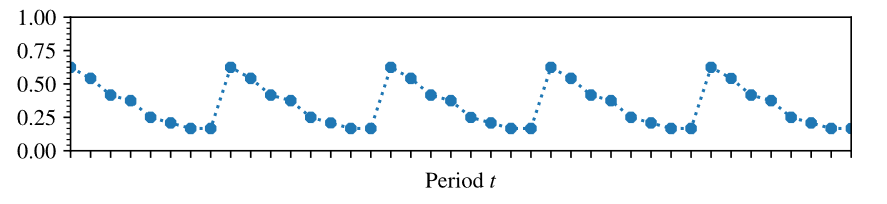
\includegraphics[width=0.7\linewidth]{pic/klein_fig7.png}
    \end{figure}

    However, unlike theoretical analysis in past works, these price cycles are deterministic: It is always the same firm that undertakes the costly action of “resetting” the price cycle by jumping up in price rather than undercutting, with the other firm able to free-ride on this.
\end{frame}

\begin{frame}{State-free Q-learning algorithm can collude}
    \cite{asker2022artificial}, \cite{asker2023impact} study the state-free Q-learning in the Bertrand model:
    \begin{enumerate}
        \item The state space for the Q-learning algorithm is reduced to a singleton, indicating that the algorithm does not rely on historical prices;
        \item $\delta=0$, implying that the algorithm considers only the one-period payoff;
        \item There is no $\epsilon$ exploration; instead, at each epoch, the agent persistently uses the greedy action;
    \end{enumerate}
    \vspace{0.2cm}

    This experiment is very \textcolor{red}{important}: $\delta=0$ implies there is no equilibrium that can collude, but the game can still converge to the supra-competitive prices.
\end{frame}

\begin{frame}{Bandit Algorithm can Collude}
    \tiny{\cite{hansen2021frontiers} assumes a linear demand:
    \[d_j^*(p_j,p_{-j})=\alpha-\beta p_j+\gamma p_{-j}.\]
    \[\pi_t(p_j,p_{-j})=p_jd_j^*(p_j,p_{-j})+\varepsilon_{j,t},\]
    \[\varepsilon_{j,t}\sim U[-\frac{1}{\delta},\frac{1}{\delta}]\]
    $\delta$ is the SNR. Both firms use a UCB-tuned algorithm to make decisions:
    \[\begin{aligned}
    \mathrm{V}_{k,t}& =\overline{{\pi_{k,t}^{2}}}-\bar{\pi}_{k,t}^{2}+\sqrt{\frac{2\log t}{n_{k,t}}}, \\
    \mathrm{UCB-tuned}_{k,t}& =\bar{\pi}_{k,t}+\sqrt{\frac{\log t}{n_{k,t}}\mathrm{min}\left(\frac{1}{4},\mathrm{V}_{k,t}\right),} 
    \end{aligned}\]}
    \begin{columns}
        \begin{column}{0.5\textwidth}
            \begin{figure}
                \centering
                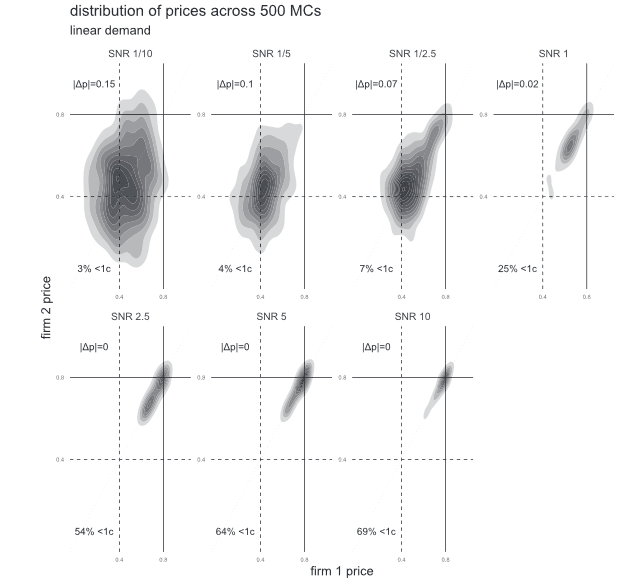
\includegraphics[width=0.7\linewidth]{pic/hansen_fig2.png}
            \end{figure}
        \end{column}
        \begin{column}{0.5\textwidth}
            \begin{figure}
                \centering
                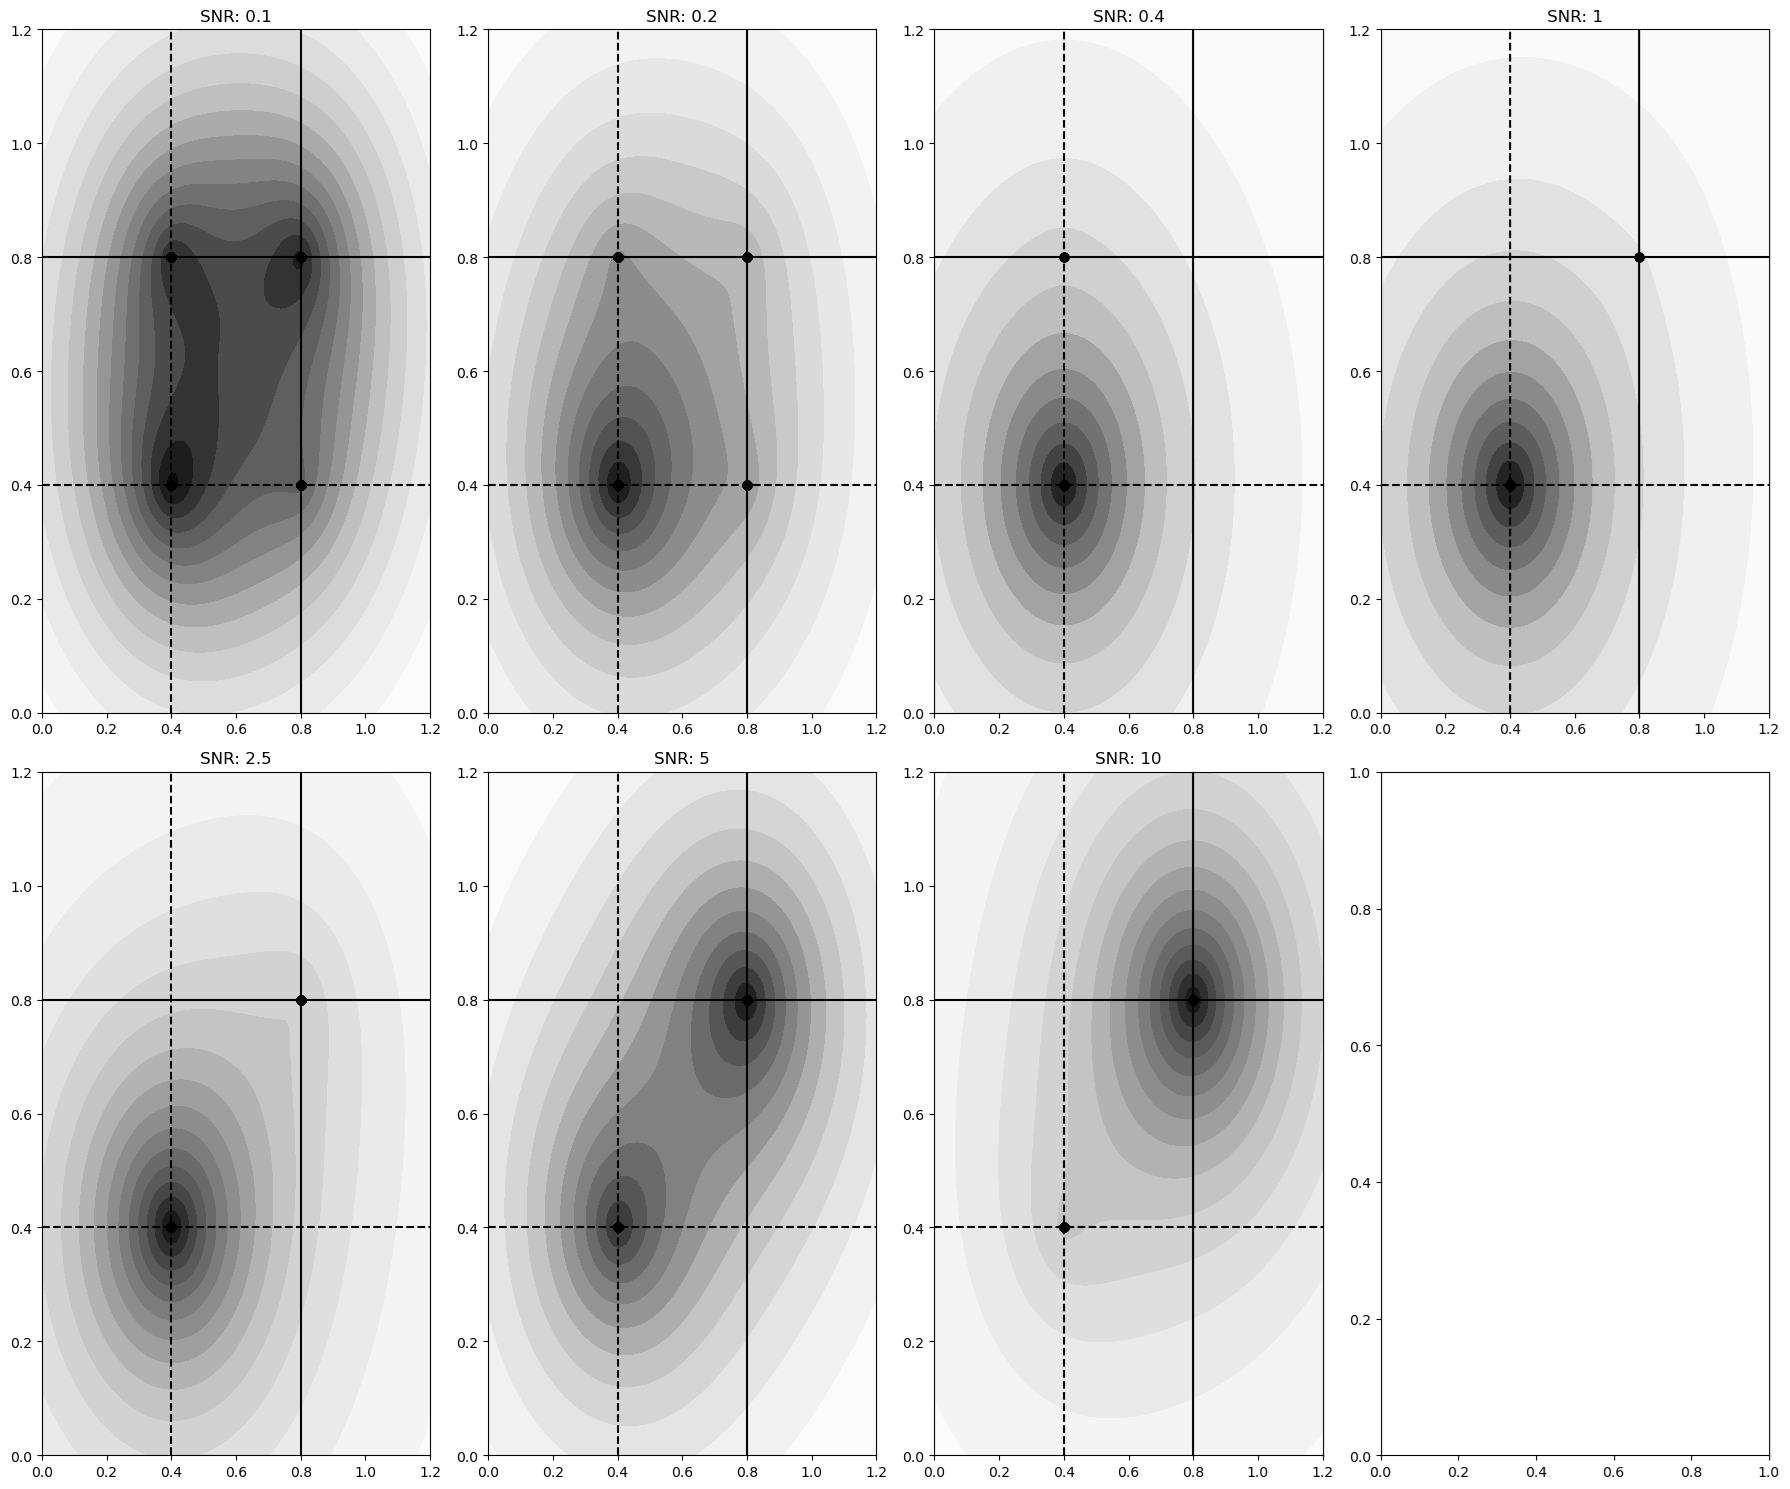
\includegraphics[width=0.7\linewidth]{pic/hansen_fig2_rep.png}
            \end{figure}
        \end{column}
    \end{columns}
\end{frame}

\begin{frame}{Other Algorithmic Collusion}
    \begin{figure}
        \centering
        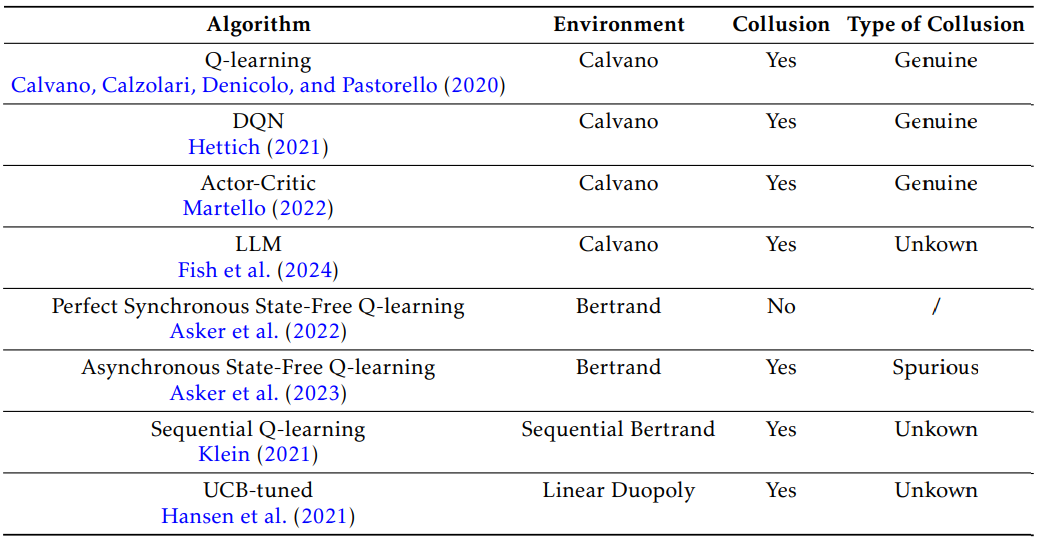
\includegraphics[width=1\linewidth]{pic/table_of_summary.png}
    \end{figure}
    In summary, between 2019 - 2022, many \textbf{numerical research} has shown that some RL algorithms can converge to collusion in the pricing game.
\end{frame}

\begin{frame}{Criticism 1: What looks like collusion need not be collusion}
    \begin{itemize}
        \item The decision made by the RL algorithm is not that `smart':
        \begin{enumerate}
            \item For example, in the research by \cite{klein2021autonomous}, the players do not exhibit the patterns exactly the same as MPE.
            \item  \cite{epivent2024algorithmic}: the algorithm will start a price war to any price modification.
        \end{enumerate}
        \item The algorithms can sometimes behave irrationally. 
    \end{itemize}
    \begin{figure}
        \centering
        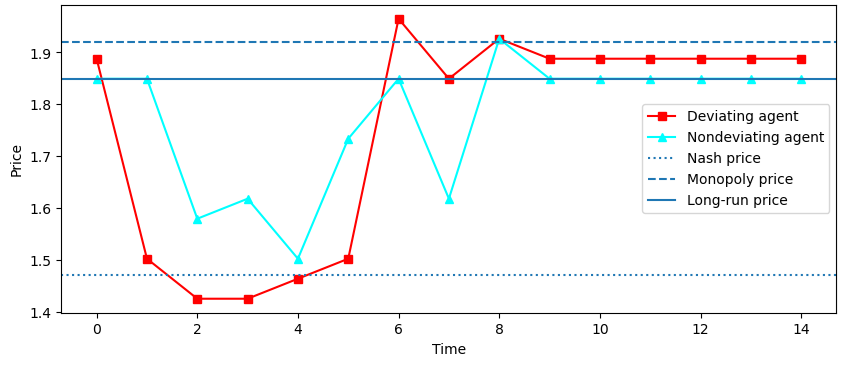
\includegraphics[width=0.5\linewidth]{pic/reward-punishment.png}
    \end{figure}
    \begin{center}
        Many scholars think these collusions are caused by the insufficient exploration inherent in the Q-learning algorithm.
    \end{center}
\end{frame}

\begin{frame}{Criticism 2 \& 3}
    \begin{enumerate}
        \item \textit{Number effect}: as the number of firms participating in the market increases, the tacit collusion induced by Q-learning may be mitigated. This phenomenon has been verified by several numerical studies including \cite{hettich2021algorithmic}, \cite{asker2022artificial}, \cite{abada2023artificial};
        \item It's not likely for firms to adopt the Q-learning algorithm to price when it can be outperformed by other simpler algorithms, such as Exp3 (\cite{den2022artificial}).
    \end{enumerate}
\end{frame}

\begin{frame}{Criticism 4: Conditions Are Harsh}

\tiny{\cite{den2022artificial} refined the definition of equilibrium to accommodate the dynamics of dynamic pricing using $\epsilon$-greedy Q-learning in a duopoly market. 

$(\delta-\epsilon)$-\textit{best-response}: A strategy $\sigma^{(i)}=\{\sigma^{(i)}(s):s\in\mathcal{A}_i\times\mathcal{A}_{-i}\}$ of player $i$ is called $(\delta-\epsilon)$-\textit{best-response} to strategy $\sigma^{(-i)}=\{\sigma^{(-i)}(s):s\in\mathcal{A}_{-i}\times\mathcal{A}_{i}\}$ if the following equation holds for all states $s$ and $s_{-i}$:
\[
    \begin{aligned}
        \sigma^{(i)}(s)&\in\arg\max_{a\in\mathcal{A}_{i}}\frac{\epsilon}{|\mathcal{A}_{-i}|}\sum_{a_{-i}\in\mathcal{A}_{-i}}\{r_{i}(a,a_{-i})+\delta V_{\sigma^{(-i)}}^{(i)}(a,a_{-i})\}\\
        &+(1-\epsilon)\{r_{i}(a,\sigma^{(-i)}(s_{-i},s_{i}))+\delta V_{\sigma^{(-i)}}^{(i)}(a,\sigma^{(-i)}(s_{-i},s_{i}))\},
    \end{aligned}
\]
where the value function $V_{\sigma(-i)}^{(i)}(s)$ is defined by:
\[
    \begin{aligned}
        V_{\sigma(-i)}^{(i)}(s)&:=\max_{p\in\mathcal{A}_{i}}\frac{\epsilon}{|\mathcal{A}_{-i}|}\sum_{a_{-i}\in\mathcal{A}_{-i}}\{r_{i}(a,a_{-i})+\delta V_{\sigma^{(-i)}}^{(i)}(a,a_{-i})\}\\
        &+(1-\epsilon)\{r_{i}(a,\sigma^{(-i)}(s_{-i},s_{i}))+\delta V_{\sigma^{(-i)}}^{(i)}(a,\sigma^{(-i)}(s_{-i},s_{i}))\},
    \end{aligned}
\]
A strtegy pair $(\sigma^{(i)},\sigma^{(-i)})$ is claled a $(\delta-\epsilon)$-\textit{strategy-equilibrium} if they are mutually $(\delta-\epsilon)$-best-response to each other. 
\vspace{0.15cm}

This definition of best response aligns with \textbf{the exploratory nature of Q-learning}. 

\vspace{0.15cm}
For any $\delta$, there exists an $\epsilon^*(\delta)\in (0,1)$ such that for all $\epsilon>\epsilon^*(\delta)$, the only $(\delta-\epsilon)$-strategy-equilibrium is both firms use the competitive price.
}
\end{frame}

\begin{frame}{Theoretical Evidence: 1}
    \begin{itemize}
        \item \cite{den2022artificial}'s $(\delta-\epsilon)$-\textit{best-response} is great and can explain the slow convergence in most numerical experiments;
        \item However, this framework takes the perspective of equilibrium rather than convergence, sometimes the game can converge to the collusive outcome even though the collusive one is not an equilibrium (\cite{asker2023impact}).
    \end{itemize}
    \vspace{0.3cm}
    \begin{center}
        To date, there is \textcolor{red}{\textbf{no universal}} conclusion on the cause of algorithmic collusion by the reinforcement learning algorithm.
    \end{center}
\end{frame}

\begin{frame}{Theoretical Evidence: 2}
    \begin{columns}[h]
        \tiny{
            \begin{column}{0.33\textwidth}
                \begin{itemize}
                \item \cite{banchio2022artificial} proposes that algorithmic collusion relies on \textit{spontaneous coupling}, which results in overestimating the Q-value of the high prices.
                \item Spontaneous coupling arises from the correlation of Q-values due to the updation being dependent on both firms' actions.
                \item This research presents sufficient conditions when spontaneous coupling does not occur (can explain some observations in \cite{asker2022artificial}.)
            \end{itemize}
            \end{column}
            \begin{column}{0.33\textwidth}
                \begin{itemize}
                    \item \cite{dolgopolov2024reinforcement} employs evolutionary game theory to analyze the convergence of \textbf{state-free} Q-learning agents in a prisoner’s dilemma game.
                    \item When both agents use logit (Boltzmann) exploration, the convergence is contingent upon a closed-form relationship between the learning rate and the payoffs.
                \end{itemize}
                \begin{figure}
                    \centering
                    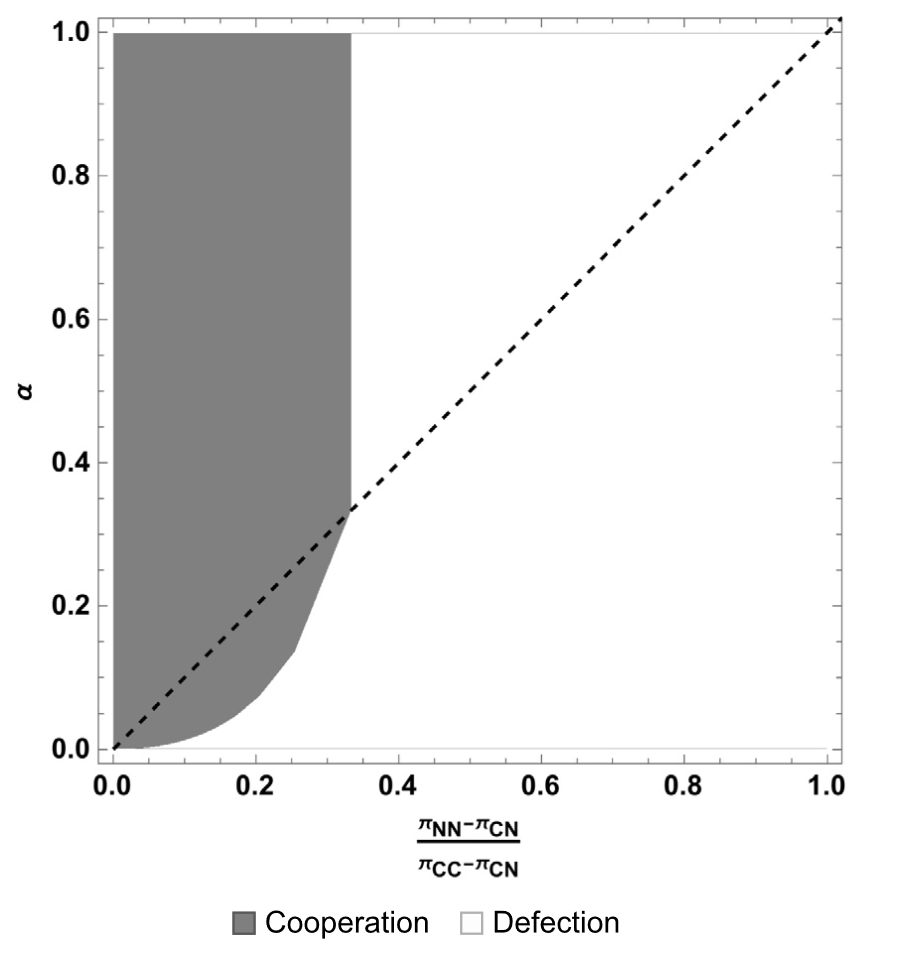
\includegraphics[width=0.75\linewidth]{pic/dolgopolov_fig2.png}
                \end{figure}
            \end{column}
            \begin{column}{0.33\textwidth}
                 \begin{itemize}
                     \item \cite{brown2023competition} examine the asymmetric setting where firms can price based on an opponent's most recent price;
                     \item It found that the price level will be supra-competitive under the MPE.
                 \end{itemize}
            \end{column}
        }
    \end{columns}
    \begin{center}
        In conclusion, under specific circumstances and parameter settings, the use of RL algorithms can \textbf{converge to} a collusive scenario with a theoretical guarantee.
    \end{center}
\end{frame}

\begin{frame}{Theoretical Evidence: 3}
    Theoretical evidence beyond reinforcement learning:
    \small{
    \begin{itemize}
        \item \cite{cho2024collusive} proved that firms using a simple model averaging and least squares estimation to price converge to a collusive scenario in a linear Bertrand duopoly setting;
        \item \cite{lamba2022pricing} studied a pricing game where firms price their goods solely based on the opponent's price during the previous epochs, it is proved that under the Markov Perfect Equilibrium, the average price set by both firms is supra-competitive;
        \item Other insights can be drawn from the theoretical studies on the collusion of Cournot games (\cite{shi2020multi}, \cite{possnig2023reinforcement}).
    \end{itemize}
    }
\end{frame}

\begin{frame}{Empirical Evidence: 1}
    The most compelling evidence comes from \cite{clark2023algorithmic}：
    \[
        y_{mt}=\alpha_m+\alpha_t+\beta_1T_{mt}^1+\beta_2T_{mt}^2+\epsilon_{mt},
    \]
    \begin{itemize}
        \item $y_{mt}$: represents the price margin in market $m$ at time $t$; 
        \item $T_{mt}^1$: dummy variable that indicate whether market $m$ at time $t$ has \textbf{only} one gas stations using algorithms to price;
        \item $T_{mt}^2$: dummy variable that indicate whether market $m$ at time $t$ has \textbf{exactly} two gas stations using algorithms to price.
    \end{itemize}
    Using instrumental variables, the authors identified that in duopoly markets, the adoption of algorithmic pricing by a single firm does not significantly affect the price margin, whereas the adoption by both firms can increase station-level margins by 28\%. 

    \begin{center}
        Algorithmic pricing can significantly increase the market prices.
    \end{center}
\end{frame}

\begin{frame}{Empirical Evidence: 2}
    \cite{wieting2021algorithms} provide an intuitive evidence:
    \begin{figure}
        \centering
        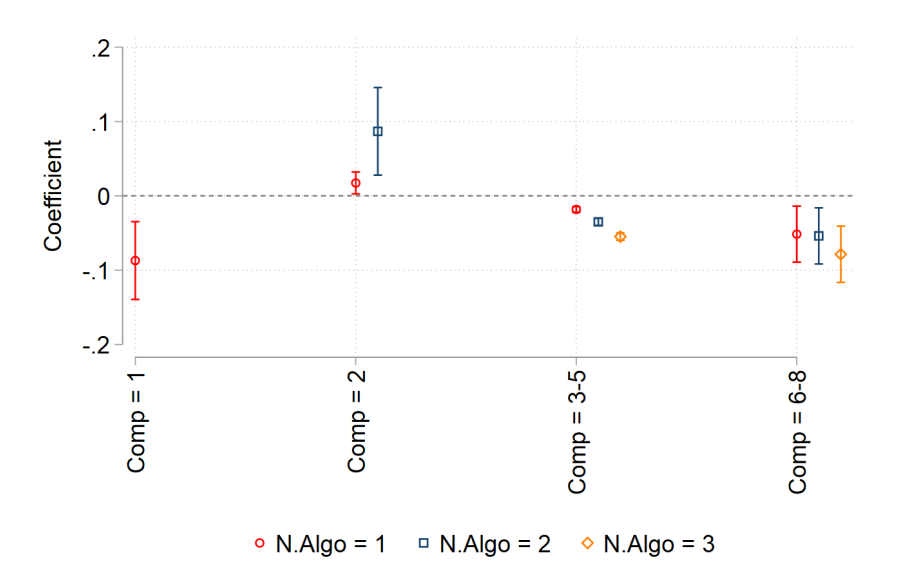
\includegraphics[width=0.5\linewidth]{pic/wieting_fig11.png}
    \end{figure}
    In a duopoly market, the adaptation of AI pricing algorithms by both firms can increase the market price.
    \begin{itemize}
        \item Another empirical evidence comes from \cite{musolff2022algorithmic};
        \item However, all empirical research only reveals that algorithmic pricing can increase the market price, not indeed to be RL algorithms.
    \end{itemize}
\end{frame}

\begin{frame}{Summary on Previous Findings}
    \begin{itemize}
        \item The reinforcement learning algorithm can result in collusive situations in many numerical experiments;
        \item The simulation can not generate a stable and `smart' enough result, some scholars question the validity of the collusion;
        \item Theoretical analysis suggests that in some settings, the Q-learning can converge to the collusion with guarantee;
        \item Empirical papers find that AI algorithms in competitive cases can increase product prices.
    \end{itemize}
\end{frame}

\begin{frame}{My Own Remarks}
    \begin{itemize}
        \item Critics may argue that the collusion, including the reward-punishment scheme, is not a well-defined equilibrium and that simple reinforcement learning;
        \item Addressing the incomplete nature of algorithmic collusion under RL is a meaningful discussion, but this does not negate the significance of algorithmic collusion under RL algorithms.
    \end{itemize}
    \vspace{0.2cm}
    \begin{center}
        \textbf{The convergence of a pricing game under RL algorithm does not need to be a theoretically well-defined equilibrium.} 
    \end{center}
    \vspace{0.2cm}
    \begin{itemize}
        \item Algorithmic collusion is a problem that deserves consideration.
    \end{itemize}
\end{frame}

\section{Authentic Algorithmic Collusion}

\begin{frame}{Definition on Authentic Collusion: 1}
    \cite{den2023mathematical} offers a fantastic framework for the duopoly game.
    \begin{itemize}
        \item Consider a repeated game between two firms, denoted by $i = 1$ and $i = -1$, selling a homogeneous product;
        \item At time $t \in \mathbb{N}$, each firm selects a price $P_{it}$ from $\mathcal{P}_i$;
        \item Demand $D_{it}, D_{-it}$ obtained by firms at time $t$ is drawn from the \textbf{unkown} demand function $d(\mathbf{P}_t)$;
        \item Each firm receives a revenue $R_{it} = P_{it} \cdot D_{it}$;
        \item The algorithm (pricing strategy) $\pi_i\in \Pi_i$ is defined as the mapping from the \textit{state} $H_{it} := (P_{is}, P_{-is}, D_{is} \, \text{ for} \, 1 \leq s \leq t)$ to the probability distribution over the action space $\mathbb{P}(\mathcal{P}_i)$.
    \end{itemize}
    We can obtain the expected cumulative reward for each firm:
    \[
        \phi_i(\pi_i,\pi_{-i},d)
    \]
    \textit{Regret} of an algorithm is defined as the difference from the reward under the \textbf{optimal fixed} action:
    \[  
        Regret_i(\pi_i,\pi_{-i},d):=\sup_{P_i^*\in \mathcal{P}_i} \phi_i(P_i^*,\pi_{-i},d) - \phi_i(\pi_i,\pi_{-i},d)
    \]
\end{frame}

\begin{frame}{Definition on Authentic Collusion: 2}
    Requirements on authentic collusion:
    \begin{enumerate}
        \item The definition of algorithm already implicitly assumes that there is no illegal communication between the two firms;
        \item Algorithmic collusion needs to achieve supra-competitive payoffs:
        \[
            \phi_i(\tilde{\pi}_i, \tilde{\pi}_{-i}, d) \geq \phi_i^{comp}(d),
        \]
        where $\phi_i^{comp}(d)$ is the expected payoff during a fully competitive setting.
        \item A `smart' collusion must have a good enough performance against alternative algorithms:
        \[
            Regret_i(\tilde{\pi}_i, \pi_{-i}, d) \leq \epsilon
        \]
        for some self-determined $\epsilon>0$.
        \item Finally, an algorithm can achieve authentic collusion if it is the best response when the opponent uses the same algorithm:
        \[
            \phi_i(\tilde{\pi}_i, \tilde{\pi}_{-i}, d) \geq \phi_i(\pi_i, \tilde{\pi}_{-i}, d)
        \]
    \end{enumerate}
\end{frame}

\begin{frame}{Definition on Authentic Collusion: Summary}
    \begin{enumerate}
        \item \textit{Spurious collusion}: No illegal communication but can achieve supra-competitive outcomes;
        \item \textit{Genuine collusion}: Based on the preceding requirements, the collusive algorithm should exhibit a reward-punishment scheme toward deviation (a subset of alternative algorithms);
        \item \textit{Authentic collusion}: Based on the preceding requirements, the collusive algorithm should have low regret against all alternative algorithms and is the best response to the collusive algorithm.
    \end{enumerate}
    \vspace{0.3cm}
    One big limitation in this paper:
    \begin{itemize}
        \item This framework does not intuitively distinguish between genuine collusion and authentic collusion; 
        \item Because it's challenging to define deviation in genuine collusion using rigorous notations.
    \end{itemize}
    \vspace{0.3cm}
    \begin{center}
        Currently, there have been two authentic algorithms.
    \end{center}
\end{frame}

\begin{frame}{Authentic Collusion 1: Composite SPSA}
    \cite{meylahn2022learning} provides the first authentic collusive algorithm. 
    
    Important Assumption in this paper:
    \begin{itemize}
        \item The demands are public information for both firms;
    \end{itemize}
    Then both firms can learn the collusive and competitive prices using Simultaneous Perturbation Kiefer–Wolfowitz recursion:
    \begin{itemize}
        \item Each firm maintains an estimation $\hat{p}_i^{col}(n)$, where $n$ is a counter；
        \item In each two consecutive times, the firm charges $\hat{p}_i^{col}(n)+c_n \omega_i^{col}(n)$ and $\hat{p}_i^{col}(n)-c_n \omega_i^{col}(n)$, $c_n$ is a tuning sequence and $\omega_i^{col}(n)$ is a random variable equals $1$ and $-1$, both with probability $\frac{1}{2}$;
        \item After observing the joint revenue $\tilde{r}^+$ and $\tilde{r}^-$ in two consecutive times, both firm take gradient descent to update $\hat{p}_i^{col}(n)$:
        \[  
            \hat{\nabla}r(n):=\frac{\tilde{r}^+ - \tilde{r}^-}{2c_{n}\omega_{i}^{col}(n)}
        \]
        \item Similarly. both firms can learn $\hat{p}_i^{com}(n)$.
    \end{itemize}
\end{frame}

\begin{frame}{Authentic Collusion 1: Composite SPSA}
    \begin{itemize}
        \item The full process includes five stages to learn the revenue under the collusive and competitive cases, then both firms decide to collude or compete based on the comparison of the revenue under the two cases;
        \item The algorithm would change to the `competitive' module if it detects the opponent is not using the algorithm to price;
        \item It is proved to be an authentic collusive algorithm.
    \end{itemize}
    \vspace{0.5cm}
    Two drawbacks of Composite SPSA:
    \begin{enumerate}
        \item It requires knowledge of the mutual demand function.
        \item The SPSA algorithm requires synchronization. i.e. if the two firms do not initiate the same algorithm simultaneously, they may not end up charging the collusive prices.
    \end{enumerate}
\end{frame}

\begin{frame}{Authentic Collusion 2: Collude-or-compete}
   \cite{loots2023data}'s \textit{Collude-or-compete} solved the above two problems.
   \[\lambda_j(\mathbf{p};\theta):=\frac{\nu_j(p_j;\theta)}{1+\nu_1(p_1;\theta)+\nu_2(p_2;\theta)}\]
   \begin{itemize}
       \item To learn the collusive price with convergence guarantee, the algorithm needs to estimate $\Theta$ consistently.
       \itme To estimate $\Theta$, both player's demand information is needed;
       \item Their algorithm can reveal the private demand information by pricing:
        \begin{enumerate}
            \item If the demand is $1$, the opponents demand is $0$;
            \item If the demand is $0$, how should we know the opponents demand,$0$ or $1$?
        \end{enumerate}
   \end{itemize}
   How to extract the demand information from the prices?
   \begin{itemize}
       \item Maintain three estimations of the parameters: $\hat{\theta}_{t,j}^{(0,0)}, \hat{\theta}_{t,j}^{(0,1)}, \hat{\theta}_{t,j}^{(1,0)}$;
       \item Calculate the collusive price $(p_{j}^{(0,0)}(t+1),p_{-j}^{(0,0)}(t+1)), (p_{j}^{(0,1)}(t+1),p_{-j}^{(0,1)}(t+1)), (p_{j}^{(1,0)}(t+1),p_{-j}^{(1,0)}(t+1))$;
       \item When $d_{t,j}=0$, assume that $d_{t,-j}=0$, and set price at $p_{j}^{(0,0)}(t+1)$;
       \item At time $t+1$, when she observes the opponent's price is $p_{-j}^{(0,1)}(t+1)$, she would know that the opponent's demand at time $t$ is $1$. 
   \end{itemize}
   The authors proved the convergence of this algorithm.
\end{frame}

\begin{frame}{Authentic Collusion 2: Collude-or-compete}
    More about the \textit{Collude-or-compete} algorithm.

    \vspace{0.5cm}
    What if the opponents choose other algorithms (not to collude)?
    \begin{itemize}
        \item The collude-or-compete includes two modules:
            \item The collude module (in the last slide) is trying to learn the parameters of the environment;
            \item The complete module can deter the opponents' incentive to use other pricing strategies.
    \end{itemize}
    \vspace{0.5cm}
    The algorithm has a mechanism to decide when to switch between the two modules, and the algorithm also has a mechanism to synchronize both firm's timing.
    
    \vspace{1cm}
    This algorithm has been proven to be an authentic collusive algorithm.
\end{frame}

\section{Regulate Algorithmic Collusion}
\label{sec:reglate}

\begin{frame}{Mutucal Impact between Algorithmic Collusion and the Market}
    \begin{columns}[h]
        \column{0.5\textwidth} 
        \begin{block}{The Market on Algorithmic Collusion}
            \begin{itemize}
                \item \cite{miklos2019collusion} found that more accurate demand forecasting algorithms can reduce potential opportunities for collusion;
                \item \cite{johnson2023platform} discovers that by restricting the size of the product assortment, the market price set by the firms using AI algorithm tends to decrease;
                \item \cite{xu2023algorithmic} verified that the occurrence of algorithmic collusion via Q-learning depends on the platform's recommendation strategy.
            \end{itemize}
        \end{block}
        \column{0.5\textwidth} 
        \begin{block}{Algorithmic Collusion on the Market}
            \cite{yang2023regulating} shows that the presence of potential algorithmic collusion can prohibit the regulator from deterring price discrimination in some settings.
        \end{block}
    \end{columns}
\end{frame}

\begin{frame}{Regulatory Measures: 1}
    Currently, there are three approaches to sustain algorithmic collusion:
    \begin{enumerate}
        \item Direct inspection of firms' pricing algorithms;
        \item Intervention in the market, where authorities act as a player with incumbent firms;
        \item Design market structures that inherently block algorithmic collusion.
    \end{enumerate}
    \vspace{0.5cm}
    The first direction is proposed by \cite{harrington2018developing} and has been more practically studied by \cite{hartline2024regulation}.
\end{frame}

\begin{frame}{Regulatory Measures: 2}
    \cite{abada2023artificial} proposes that the regulator can participate in the market itself.
    \begin{itemize}
        \item Specifically, the regulator can implement a simple reward-punishment strategy: bidding aggressively when the market appears collusive and bidding conservatively when the market appears competitive (this paper studies the circumstance of the electricity trading market). 
        \item Numerical results indicate that this strategy can substantially enhance market welfare. The blue line represents the regulator using the reward-punishment strategy and the green line represents the three-firm competing scenario.
    \end{itemize}
    \begin{figure}
        \centering
        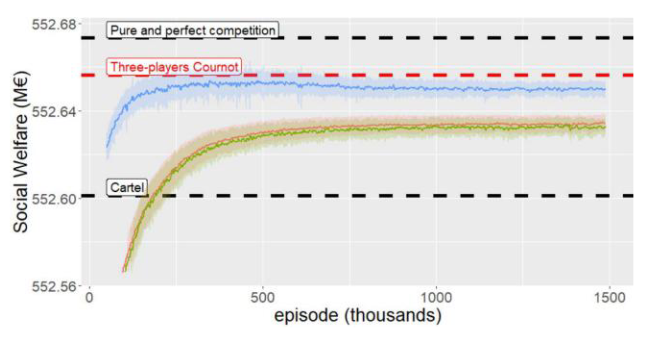
\includegraphics[width=0.45\linewidth]{pic/abada_fig7.png}
    \end{figure}
    \begin{itemize}
        \item The authors also test alternative strategies: the regulator can employ the same Q-learning algorithm, but instead of using the payoff as the reward, the regulator updates Q-values using the welfare. However, this approach has little impact on alleviating algorithmic collusion.
    \end{itemize}
\end{frame}

\begin{frame}{Regulatory Measures: 3}
    \cite{johnson2023platform} centers on strategies to deter algorithmic collusion for platform owners. 
    \begin{itemize}
        \item Consider a platform where multiple firms employ Q-learning to set their prices, while the platform determines the assortment of products recommended to consumers;
        \item The authors propose two recommendation principles that can deter algorithmic collusion:
        \begin{enumerate}
            \item Limit the size of the assortment. 
            \item Recommend the lowest-priced product first, and if no other firm offers products with a significantly lower price, then never recommend the products of other firms.
        \end{enumerate}
    \end{itemize}
    \begin{figure}[ht]
        \centering
        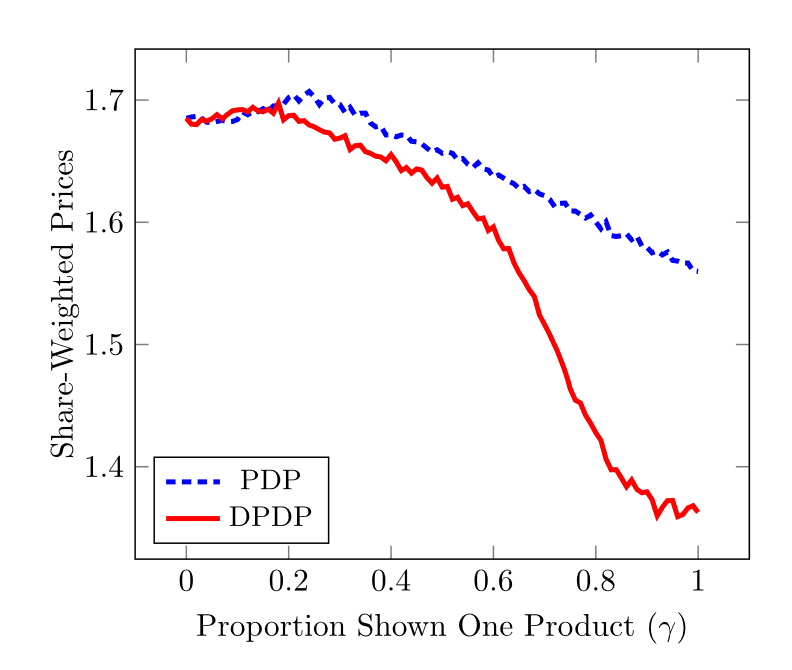
\includegraphics[width=0.4\linewidth]{pic/johnson_fig5.png}
    \end{figure}
    \end{frame}

\section{Conclusions}

\begin{frame}{Summary \& Conclusions}
    \small{
    \begin{enumerate}
        \item Many numerical studies have demonstrated that Q-learning and some other reinforcement learning algorithms can lead to supra-competitive prices in oligopoly pricing games.
        \item Some theoretical work proves that, under appropriate parameters, Q-learning (as well as some other algorithms) can converge to collusive prices in certain simple settings. Some of the convergences achieved are well-defined equilibriums, whereas the majority are not.
        \item Empirical evidence has identified that algorithmic pricing (not necessarily RL algorithms) can increase prices under competitive conditions;
        \item Although the current evidence is incomplete, and the seeming collusion is widely believed to be due to imperfect exploration, it still poses a great threat to social welfare because algorithmic collusion does not need to be a theoretically well-defined equilibrium; it just happens there.
        \item Collusions observed under RL algorithms can be categorized as spurious or genuine based on whether they exhibit a reward-punishment scheme for deviation. However, these types of algorithms can be outperformed by alternative algorithms, making them not likely to be practiced.
        \item Authentic collusion is a robust definition of algorithmic collusion, which must perform well against all alternative algorithms and be the best response toward itself (This has been beyond the scope of reinforcement learning). 
        \item Authentic collusive algorithms have been developed, but current versions require to know (or infer) the opponent's demand information. 
        \item Algorithmic collusion can be mitigated by the number effect. Regulatory intervention through active participation in the market, employing a reward-punishment strategy, can largely eliminate collusion.
    \end{enumerate}
    }
\end{frame}

\begin{frame}{Further Research: 1}
    \tiny{
    \begin{columns}[T]
        \column{0.33\textwidth} 
        \begin{block}{Numerical Research}
            \begin{itemize}
                \item Incorporating constraints such as inventory cost and strategic consumer behaviors can make the simulations more representative of reality;
                \item Current numerical research only uses `static strategies', using molecular strategies (\cite{kimbrough2005learning}) can make the results more explainable;
                \item Can AI algorithm lead to price discrimination and unfair pricing in other environments (\cite{spann2024algorithmic})?
                \item Algorithmic collusion in other fields (\cite{contDynamicsMarketMaking2024}, \cite{gu2023can}).
            \end{itemize}
        \end{block}
        \column{0.33\textwidth} 
        \begin{block}{Emirical Research}
            \begin{itemize}
                \item Identify the number effect;
                \item The mutual impact between the market structure and algorithmic collusion;
                \item Current empirical research has identified instances of algorithmic collusion, but the algorithms in these studies are only AI algorithms, not necessarily RL algorithms.
            \end{itemize}
        \end{block}
        \column{0.33\textwidth} 
        \begin{block}{Theretical Research}
            \begin{itemize}
                \item A more rigorous framework to differentiate genuine collusion and authentic collusion;
                \item Future work could aim to provide more robust proofs of the convergence of Reinforcement Learning algorithms to collusive outcomes;
                \item Current authentic collusive algorithms need to infer the opponent's demand information; future research could design collusive algorithms without relying on this channel.
            \end{itemize}
        \end{block}
    \end{columns}
    }
\end{frame}

\begin{frame}{Further Research: 2}
    \small{
    Other research directions:
    \begin{itemize}
        \item Research on the regulating aspect is lacking. Although in settings where a platform acts as an intermediary to determine which products are accessible to consumers, there are relatively practical solutions to deter algorithmic collusion (\cite{johnson2023platform}); However, in settings where products are directly accessible to consumers without platform filtration, regulatory measures have a huge potential to be investigated (\cite{harrington2018developing}, \cite{abada2023artificial}, \cite{hartline2024regulation});
        \item The recommender systems described in \cite{johnson2023platform}, \cite{xu2023algorithmic} may be more accurately modeled by assortment optimization problems in the OM literature. Under the current assortment optimization model, what will the market dynamics converge to when sellers use RL algorithms to price?
        \item Future studies could devise the optimal coupon distribution strategy or explore alternative market structure modifications to improve platform payoffs and social welfare. 
    \end{itemize}
    }
\end{frame}

\begin{frame}{Q\& A}
    \begin{center}
      {\Hugek Any Questions?}
  \end{center}
\end{frame}

\begin{frame}
  \begin{center}
      {\Hugek Thanks!}
  \end{center}
\end{frame}

\section{Reference}

\begin{frame}[allowframebreaks]
  \bibliography{reference}
  \bibliographystyle{apalike}
\end{frame}

\end{document}
